\subsubsection{Ingress}
\label{subsec:kubernetes:ingress}
Ingress Objekte dienen dem externen Zugriff auf Anwendungen in einem Cluster.
Hierbei werden HTTP und HTTPS Routen freigegeben, 
welche auf Service Objekte innerhalb des Cluster verweisen.
Routen können basierend auf Pfaden oder Host-Headern an verschiedene Service Objekte und somit Pods verteilt werden \cite{kubernetesIngress}.
Dargestellt wird dieser Kommunikationsfluss in \ref{fig:ingress_communication}.

\begin{figure}[h]
  \centering
  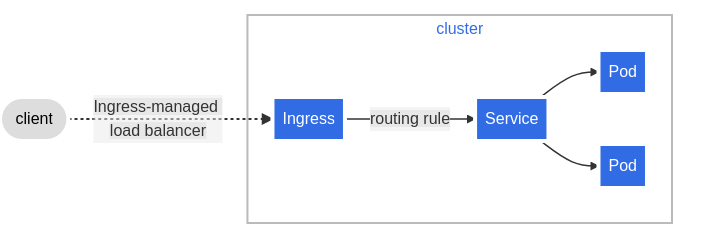
\includegraphics[width=\textwidth]{gfx/chapters/2_grundlagen/ingress.png}
  \caption{Ingress Kommunikation im Cluster}
  \label{fig:ingress_communication}
  \source{\cite{kubernetesIngress}}
\end{figure}

Kubernetes selbst definiert keinen Standard Controller zum Verwalten von Ingress Objekten \cite{Burns2019}.
Nutzer müssen selbst dafür sorgen einen Ingress Controller, 
wie beispielsweise den Nginx Ingress Controller (siehe \ref{sec:komponenten:externe-apps}), zu installieren \cite{Burns2019}.

Zur Verschlüsselung der Kommunikation können Ingress Objekten eine TLS Konfiguration übergeben werden.
Hierfür werden SSL Zertifikate sowie Schlüssel in Secret Objekten (siehe \ref{subsec:kubernetes:configmap_secret}) gespeichert und im
Ingress Objekt referenziert. 
Zur Vereinfachung der Verwaltung dieser Zertifikate können Projekte wie \emph{Cert-Manager} (siehe \ref{sec:komponenten:externe-apps})
genutzt werden, welche die Verwaltung übernehmen \cite{Burns2019}.